%! Author = dayan3847
%! Date = 11/09/23

% Preamble
\documentclass{beamer}
% Packages
\usepackage{amsmath}
\usepackage{graphicx}
\usepackage{blkarray}

\setbeamertemplate{navigation symbols}{}

\setbeamercolor{frametitle}{fg=black,bg=white}
\setbeamercolor{title}{fg=black,bg=yellow!85!orange}
\usetheme{AnnArbor}
\beamersetuncovermixins{\opaqueness<1>{25}}{\opaqueness<2->{15}}

\title{Bayes Estimation}
\subtitle{\textsc{Practice 2}}
\author[Dayan \& Mario]
{
    \authorcr\textsc{Ing.}~Dayan~\textsc{Bravo~Fraga}\inst{1}\\
    \and
    \authorcr\textsc{Ing.}~Mario~\textsc{Herrera~Almira}\inst{2}\\
    \vspace{.5cm}
    \emph{Teacher:}\\
    \and
    \authorcr\textsc{Dr.}~Arturo~\textsc{Espinosa~Romero}\inst{3}\\
}

\logo{
    
\includegraphics[scale=.1]{./img/logo_uady}
}
\institute[UADY]{
    \begin{center}
        \textbf{MCC}\\
        \textbf{Facultad de Matemáticas}\\
        \textbf{Universidad Autónoma de Yucatán}\\
    \end{center}
}
\date[September 2023]{September 2023}

% Document
\begin{document}
    \begin{frame}
        \label{frm:titlepage}
        \titlepage
    \end{frame}

    \begin{frame}
        \frametitle{Table of contents}
        \tableofcontents
    \end{frame}


    \section{Expected value}\label{sec:expected_value}
    \begin{frame}
    \Huge
    \begin{center}
        \textbf{Expected Value}
    \end{center}
\end{frame}

\subsection{Definition}\label{subsec:definition}
\begin{frame}
    \frametitle{Definition}
    \begin{block}{}
        The expected value of a random variable $X$ is the weighted average of the possible values that $X$ can take, each value being weighted according to the probability of that event occurring.
    \end{block}
\end{frame}
\begin{frame}
    \frametitle{Definition}
    \begin{block}{}
        In probability theory, the expected value (also called expectation, expectancy, expectation operator, mathematical expectation, mean, average, or first moment) is a generalization of the weighted average.
        Informally, the expected value is the arithmetic mean of a large number of independently selected outcomes of a random variable.
    \end{block}
\end{frame}

\subsection{Notations}\label{subsec:notations}
\begin{frame}
    \frametitle{Notations}
    \begin{block}{}
        The expected value of a random variable $X$ is often denoted by $E[X]$, $E(X)$, or $EX$
    \end{block}
    \begin{block}{}
        \begin{itemize}
            \item $E[X]$: Expected value of $X$.
            \item $E[X|Y]$: Expected value of $X$ given $Y$.
            \item $E[X|Y=y]$: Expected value of $X$ given $Y=y$.
        \end{itemize}
    \end{block}
\end{frame}

\subsection{Discrete case}\label{subsec:equation}
\begin{frame}
    \frametitle{Equation: Discrete case}
    For a discrete random variable $X$ with probability function $P[X=x_i]$, with $i=1,2,\dots,n$, the expected value of $X$ is defined as:
    \begin{block}{}
        \begin{equation}
            E[X] = \sum_{i=1}^{n} x_i P[X=x_i]\label{eq:equation1}
        \end{equation}
    \end{block}
\end{frame}

\subsection{Example}\label{subsec:example}
\begin{frame}
    \frametitle{Example}
    \begin{block}{}
        Let $X$ represent the outcome of a roll of a fair six-sided die.
        More specifically, $X$ will be the number of pips showing on the top face of the die after the toss.
        The possible values for $X$ are 1, 2, 3, 4, 5, and 6, all of which are equally likely with a probability of $\frac{1}{6}$.\\
        The expectation of $X$ is ``$3.5$''.
    \end{block}
    \begin{equation}
        E[X] = \sum_{i=1}^{6} x_i \frac{1}{6} = 1 \cdot \frac{1}{6} + 2 \cdot \frac{1}{6} + 3 \cdot \frac{1}{6} + 4 \cdot \frac{1}{6} + 5 \cdot \frac{1}{6} + 6 \cdot \frac{1}{6} = 3.5\label{eq:equation2}
    \end{equation}
\end{frame}

\subsection{Proof}\label{subsec:proof}
\begin{frame}
    \frametitle{Proof}
    An illustration of the convergence of sequence averages of rolls of a die to the expected value of 3.5 as the number of rolls (trials) grows.
    \begin{figure}[h]
        \centering
        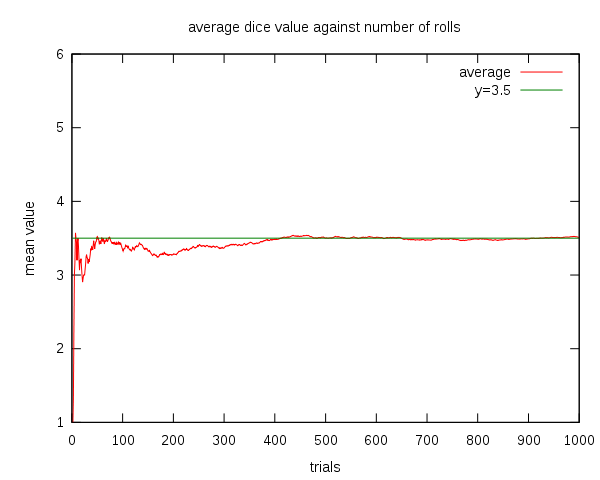
\includegraphics[width=0.5\linewidth]{./img/600px-Largenumbers.svg}
        \caption{Average of 1000 rolls of a die.}
        \label{fig:example1}
    \end{figure}
\end{frame}

\subsection{Continuous case}\label{subsec:continuous}
\begin{frame}
    \frametitle{Equation: Continuous case}
    For a continuous random variable $X$ with probability density function $f(x)$, the expected value of $X$ is defined as:
    \begin{block}{}
        \begin{equation}
            E[X] = \int_{-\infty}^{\infty} x f(x) dx\label{eq:equation3}
        \end{equation}
    \end{block}
\end{frame}

\subsection{Sum of Expectations}\label{subsec:sum}
\begin{frame}
    \frametitle{Sum of Expectations}
    \begin{block}{}
        If $X$ and $Y$ are independent random variables, then the expected value of the sum of $X$ and $Y$ is equal to the sum of their expected values:
        \begin{equation}
            E[X+Y] = E[X] + E[Y]\label{eq:equation4}
        \end{equation}
    \end{block}
\end{frame}


    \section{Conditional probability}\label{sec:conditional_probability}
    \begin{frame}
    \Huge
    \begin{center}
        \textbf{Conditional Probability}
    \end{center}
\end{frame}

\subsection{Definition}\label{subsec:definition2}
\begin{frame}
    \frametitle{Definition}
    \begin{block}{}
        In probability theory, conditional probability is a measure of the probability of an event occurring, given that another event (by assumption, presumption, assertion or evidence) has already occurred.
    \end{block}
\end{frame}
\begin{frame}
    \frametitle{Definition}
    \begin{block}{}
        The conditional probability of an event $A$ given that another event $B$ has occurred is the probability of $A$ given $B$:
        \begin{equation}
            P[A|B] = \frac{P[A \cap B]}{P[B]}\label{eq:equation21}
        \end{equation}
    \end{block}
\end{frame}



\end{document}
